\documentclass[]{article}

\usepackage{float}
\usepackage{graphicx}

\usepackage[colorlinks]{hyperref}
\usepackage[acronym]{glossaries}


\title{Technical Design Report \\
	\large Software for Science - CERN Load Balancing}

\author{\textbf{Team 6 Hexoxide} \\
	Eloy Maduro Clement \\
	Geoffrey van Driessel \\
	Corne Lukken \\
	Bram Tukker}

\date{\textbf{\today} \\
	v1.0}


\makenoidxglossaries
\newacronym{ALICE}{ALICE}{A Large Ion Collider Experiment}
\newacronym{LS2}{LS2}{Long Shutdown 2}
\newacronym{AUAS}{AUAS}{Amsterdam University of Applied Sciences}
\newacronym{TDR}{TDR}{Technical Design Report}
\newacronym{SSH}{SSH}{Secure Shell}
\newacronym{NAT}{NAT}{Network Address Translation}

\begin{document}

\maketitle
\newpage


\section{Introduction}

This document reflects the discovered \& analysed technical components for the CERN Load Balancing project. Components are identified in previously available documents as well as discoveries of the project team itself.

This is the initial version of the technical design report and the main focus will be on hardware specification of the pi cluster, setup of the initial cluster and the conducted experiments on the cluster.


\section{Hardware Specifications}

According to the \acrfull{ALICE} \hyperref[sec:ref01]{\acrfull{TDR} [1]}, there will be two types of computing nodes in the O2 project after \acrfull{LS2}. In total there will be about 2000 nodes in O2, 250 so called FLP nodes and 1750 EPN nodes.

A set of 80 computing devices grouped in units of four has been provided by the \acrfull{AUAS} for this project. These 80 nodes will be used to simulate network scenarios as close as possible to the actual O2 computing network. The computing devices at \acrshort{AUAS} will be Raspberry Pi’s, specifically, model 3 B+.

In table 1 a comparison of differences in hardware is detailed. It is clear that the computing nodes provided by \acrshort{AUAS} are vastly inferior to the computing hardware that will become available for \acrshort{ALICE} O2. These hardware differences must be taken greatly into account during the project and its various experiments.

\begin{table}[H]
	\begin{center}
		\begin{tabular}{ | l | l | l | l | }
			\hline
			Component & FLP (250) & EPN (1750) & Raspberry Pi 3 B+ (80) \\ \hline
			CPU & ? x86 & 32 Core x86 & 4 Core ARMv8 \\ \hline
			RAM & 32GB & 128GB & 1GB \\ \hline
			Ethernet & 4 x 10GB & 10GB & 300MB \\
			\hline
		\end{tabular}
		\caption{Hardware specifications of computing nodes.}
		\label{tab:specs}
	\end{center}
\end{table}


\section{Setup Pi Clusters}

The pi clusters were initially empty. So the pi clusters had to be setup with an image. To increase the initialise process, one image was made and reused for the other clusters. The required dependencies were also installed on the initial image. A bash script was developed which helps with the installation of the dependencies. The remaining processes were automated with Ansible.

\subsection{Software}
An environment as similar as possible to the one used at CERN is desired, however, it has proven to be not feasible to use CentOS. This is due to the limitations the Raspberry pi version has in comparison to the CentOS x86\_64 image. One of the main reasons is the inability to switch of gcc version, normally, a tool called scl provides the switching for specific versions of many development tools. The version of gcc supplied with CentOS is incompatible with the version of boost that is specified in many of the previous experiments. Furthermore the version of gcc is not capable of compiling c++2011 features which is required by CERN. To continue to use CentOS gcc would have to be built to be build from source.

To resolve the issues with the CernOS image an alternative had to be elected. Based on previous experience Manjaro 17.1 was chosen, Manjaro provides a full features ARM image for which a tremendous amount of packages are available. Manjaro being an Arch based distribution is extremely permissive in adaptive configurations allowing it to closely reflect any other distribution.

Based on the reports of the previous experiments, here follows a list of dependencies that were installed on the pi’s:

\begin{table}[H]
	\begin{center}
		\begin{tabular}{ | l | l | l |}
			\hline
			Library/Tool & Version required & Version specified \\ \hline
			FairMQ & 1.1.5 & 1.1.5 \\ \hline
			ZeroMQ & 4.2.2 & 4.2.1 \\ \hline
			Zookeeper & 3.4.9 & 3.4.9 \\ \hline
			Cmake & 3.11.0 & 3.11.0 \\ \hline
			Boost & 1.66.0 & 1.66.0 \\ \hline
			Yaml-cpp & 0.5.2 & 0.5.2 \\ \hline
			FairLogger & 1.0.6 & NONE \\ \hline
			Compiler & gcc 8.2.0 & gcc 6.3.0 \\
			\hline
		\end{tabular}
		\caption{The installed software dependencies on the pi’s.}
		\label{tab:librabies}
	\end{center}
\end{table}

To make our experiments reproducible, a \hyperref[sec:ref02]{bash script [2]} was made which will install all the dependencies automatically.

\subsection{SSH}
During the first phase of the project remote access to a pi cluster through \acrshort{SSH} was configured. Having access to pi nodes is of advantage as team members can now access a node at any time and location.

The team member Corne has setup the pi cluster within his home network. Through network segregation, it is ensured that no one can access any other systems that are connected to the network. 

The network segregation is done by using \acrfull{NAT}.
Since the pi cluster has four individual pi’s, four different (none default) ports are forwarded. This way, each port will access a different pi in the cluster.

Lastly, since the network address is public, it is important that only authorized persons can access the pi’s. To ensure this a secure ssh password was configured.

\begin{center}
	\begin{figure}[H]
		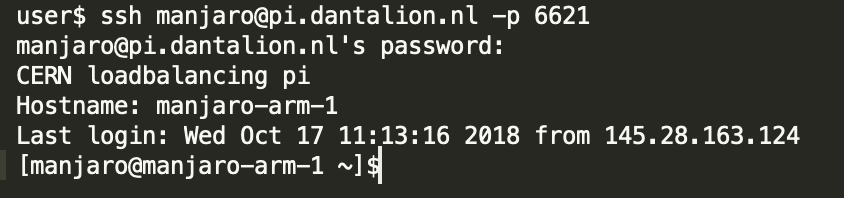
\includegraphics[width=\textwidth]{SSH}
		\caption{Example of login in using \acrshort{SSH} on remote accessible raspberry pi.}
		\label{fig:ssh}
	\end{figure}
\end{center}

\subsection{Ansible}
To run and configure tests on the pi clusters, some things will need to be configured. Ansible will be used to handle the configuration of each pi's hostname, defining which experiments to run and with which parameters to do so. Furthermore, Ansible brings extensive logging capabilities with which the metrics below will be monitored real-time.

\begin{table}[H]
	\begin{center}
		\begin{tabular}{ | c | }
			\hline
			Metric \\ \hline
			Temperatures \\ \hline
			Throughput \\ \hline
			Scaling governer / Core clock \\ \hline
			Memory usage \\ \hline
			CPU usage \\ \hline
			Swap \\ \hline
			Fail-over \\
			\hline
		\end{tabular}
		\caption{Metric that will be used in the experiments with Ansible.}
		\label{tab:specs}
	\end{center}
\end{table}


\section{Experiments}

In order to get familiar with the hardware of the pi clusters, the experiments from \hyperref[sec:ref03]{Heiko [3]} will be replicated. The experiments were performed in the following order:
\begin{itemize}
	\item Experiment 1: Ticktime influence on both algorithms with one fail-over
	\item Experiment 2: Ticktime influence on both algorithms with all but one fail-over
	\item Experiment 3: Experiment 2 with random sample size
\end{itemize}

\printnoidxglossary[type=\acronymtype]


\begin{thebibliography}{}
	\label{sec:ref01}\bibitem{}\href{http://cds.cern.ch/record/2011297/files/ALICE-TDR-019.pdf?version=3}{ALICE Technical Design Report}
	\label{sec:ref02}\bibitem{}\href{https://github.com/hexoxide/raspberry-dependency}{raspberry-dependency}
	\label{sec:ref03}\bibitem{}\href{https://github.com/hexoxide/O2-Balancer}{O2-Balancer}
\end{thebibliography}


\end{document}
